\section*{branch prediction more generally}

\begin{comment}
\begin{frame}{interlude: real processors}
% FIXME: intro: real branch prediction a lot more complicated
% FIXME: die photo branch prediction logic
\end{frame}
\end{comment}

\begin{frame}[fragile,label=betterPredict]{better branch prediction}
\begin{itemize}
\item forward (target $>$ PC) not taken; backward taken
\item intuition: loops:
\end{itemize}
\begin{lstlisting}[style=small]
LOOP: ...
      ...
      je LOOP

LOOP: ...
      jne SKIP_LOOP
      ...
      jmp LOOP
SKIP_LOOP:
\end{lstlisting} 
\end{frame}

\begin{frame}{predicting ret: extra copy of stack}
\begin{itemize}
    \item predicting ret --- stack in processor registers
    \item different than real stack/out of room? just slower
\end{itemize}
\begin{tikzpicture}
\matrix [matrix of nodes, nodes={draw,rectangle,row sep=-\pgflinewidth,font=\scriptsize, text width=3cm},
         label={-90:stack in memory}] (realStack) {
    baz saved registers \\
    baz return address \\
    bar saved registers \\
    bar return address \\
    foo local variables \\
    foo saved registers \\
    foo return address \\
    foo saved registers \\
 };

\matrix [matrix of nodes,row sep=-\pgflinewidth,nodes={draw,rectangle,font=\scriptsize,text width=3cm},
         label={[align=center]-90:(partial?) stack\\in CPU registers},right=1cm of realStack] (fakeStack) {
    baz return address \\
    bar return address \\
    foo return address \\
 };
\end{tikzpicture}
\end{frame}

\begin{frame}{prediction before fetch}
\begin{itemize}
    \item real processors can take \myemph{multiple cycles} to read instruction memory
    \item predict branches \myemph{before reading their opcodes}
    \item how --- more extra data structures
        \begin{itemize}
            \item tables of recent branches (often many kilobytes)
        \end{itemize}
\end{itemize}
\end{frame}

% FIXME: ...
\begin{frame}{2004 CPU}
    \begin{tikzpicture}[scale=1.25]
\clip (1,0) rectangle (13, 7);
\node[anchor=south west] (diePhoto) at (0,0) {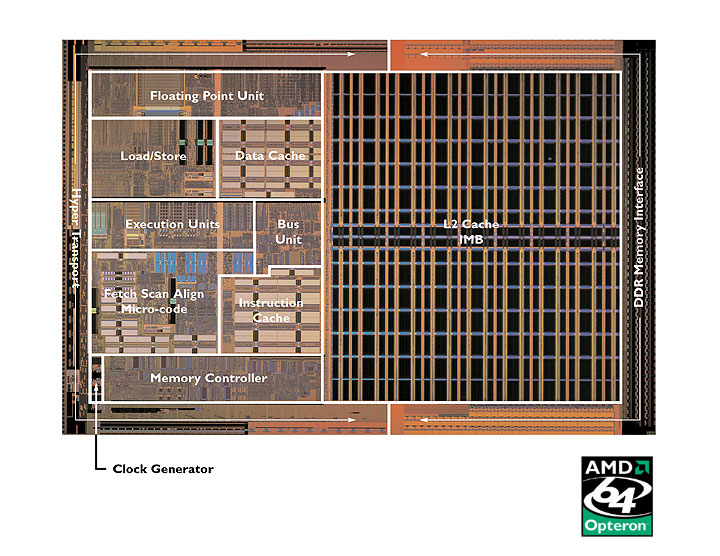
\includegraphics[width=11.25cm]{../pipe/Opteron_die_labelled.jpg}};
%\draw[red] (0, 0) grid (9,7);
    \draw[fill=red,opacity=0.6] (1.9,6.2) rectangle (2.4,5.8);
    \draw[fill=red,opacity=0.6] (1.7,4.2) rectangle (1.9,4.6);

    \draw[fill=red!60!white] (10,7) -- (9.75,6.5) -- (10.25,6.5) -- cycle;
    \node[anchor=west] at (10.1, 6.75) {Registers};
    %\draw[fill=orange,opacity=0.6] (2.95,2.7) rectangle (4.2,3.6);
    \draw[fill=orange,opacity=0.6] (2.95,2.7) -| (4.2,3.8) -| (3.6,3.65) -- (2.95,3.65) -- (2.95,2.7);
    \draw[fill=orange,opacity=0.6] (2.95,4.6) rectangle (4.2,5.6);

    \draw[fill=orange!60!white] (9.5,6) -- (9.75,6.5) -- (10.25,6.5) -- (10.5,6) -- cycle;
    \node[anchor=west] at (10.35,6.25) {L1 cache};
    \draw[fill=yellow,opacity=0.6] (4.2,2.1) rectangle (7.9,6.25);
    
    \draw[fill=yellow!60!white] (9.25,5.5) -- (9.5,6) -- (10.5,6) -- (10.75,5.5) -- cycle;
    \node[anchor=west] at (10.6,5.75) {L2 cache};

    \draw[fill=blue,opacity=0.6] (2.87,2.7) -- (2.35, 2.7) -- (2.35, 3.55) -- (2.5, 3.55) -- (2.5, 3.0) -| cycle;
        \begin{scope}[xshift=-1cm]
        \draw[fill=blue,opacity=0.6] (1.45, 3.4) rectangle (1.9, 3.75);
        \node[anchor=west,align=left] at (10.6,3) {Branch Prediction \\ (approximate)};
    \draw[fill=blue!60!white] (10.1,3.25) rectangle (10.5, 2.75);
        \end{scope}
\end{tikzpicture}
    \imagecredit{Image: approx 2004 AMD press image of Opteron die; \\ approx register/branch prediction location via chip-architect.org (Hans de Vries)}
\end{frame}
